
\documentclass[a4paper,UKenglish,cleveref, autoref, thm-restate]{lipics-v2021}
%This is a template for producing LIPIcs articles. 
%See lipics-v2021-authors-guidelines.pdf for further information.
%for A4 paper format use option "a4paper", for US-letter use option "letterpaper"
%for british hyphenation rules use option "UKenglish", for american hyphenation rules use option "USenglish"
%for section-numbered lemmas etc., use "numberwithinsect"
%for enabling cleveref support, use "cleveref"
%for enabling autoref support, use "autoref"
%for anonymousing the authors (e.g. for double-blind review), add "anonymous"
%for enabling thm-restate support, use "thm-restate"
%for enabling a two-column layout for the author/affilation part (only applicable for > 6 authors), use "authorcolumns"
%for producing a PDF according the PDF/A standard, add "pdfa"

%\pdfoutput=1 %uncomment to ensure pdflatex processing (mandatatory e.g. to submit to arXiv)
%\hideLIPIcs  %uncomment to remove references to LIPIcs series (logo, DOI, ...), e.g. when preparing a pre-final version to be uploaded to arXiv or another public repository

%\graphicspath{{./graphics/}}%helpful if your graphic files are in another directory

\usepackage{cite}
\usepackage{amsmath,amssymb,amsfonts}
\usepackage{algorithmic}
\usepackage{graphicx}
\usepackage{bussproofs}
\EnableBpAbbreviations
\usepackage{hyperref}
\usepackage{tikz,pgfplots}
\pgfplotsset{compat=newest}
\usepackage{tikz-cd}
\usepackage{textcomp}
\usepackage{xcolor}
\usepackage{amsthm}
\usepackage{caption}
\usepackage{subcaption}
\usetikzlibrary{cd}
\usepackage{mathabx}
\usepackage{cmll}
\usepackage{stmaryrd}
\usepackage{wrapfig}
\usepackage{relsize}

\input{prooftree}

\usepackage{proof}

\bibliographystyle{plainurl}% the mandatory bibstyle



% MATH TEXT STYLES
\newcommand{\B}[1]{\mathbf{#1}}
\newcommand{\BB}[1]{\mathbb{#1}}
\newcommand{\C}[1]{\mathcal{#1}}
\newcommand{\F}[1]{\mathfrak{#1}}
\newcommand{\TT}[1]{\mathtt{#1}}
\newcommand{\RM}[1]{\mathrm{#1}}
\newcommand{\SF}[1]{\mathsf{#1}}



%CATEGORIES

\newcommand{\Met}{\mathsf{Met}}
\newcommand{\Mod}{\Lawv\mathsf{Mod}}
\newcommand{\GMet}{\Lawv\mathsf{CCat}}
\newcommand{\Fun}{\mathsf{Fun}}
\newcommand{\colim}{\mathrm{colim}}
\newcommand{\Yon}{\B{Y}}
\newcommand{\Hom}{\mathrm{Hom}}
\newcommand{\Sym}{\mathrm{Sym}}
\newcommand{\matr}[1]{\hat{#1}}

\newcommand\pfun{\mathrel{\ooalign{\hfil$\mapstochar\mkern5mu$\hfil\cr$\to$\cr}}}



% LAMBDA CALCULI

\newcommand{\lamcalc}{$\lambda$-calculus}
\newcommand{\lam}{\lambda}

\newcommand{\STLC}{\RM{STLC}}
\newcommand{\BSTLC}{\mathsf b\RM{STLC}}
\newcommand{\RSTLC}{\C R\RM{STLC}}
\newcommand{\STDLC}{\RM{ST}\partial\RM{LC}}
\newcommand{\Real}{\SF{Real}}

\newcommand{\Der}{\SF D}
\newcommand{\To}{\Rightarrow}

\newcommand{\finMS}[1]{\C M_{\RM{fin}}(#1)}

\newcommand{\true}{\RM{True}}
\newcommand{\false}{\RM{False}}
\newcommand{\bool}{\SF{Bool}}

\newcommand{\Te}[1]{\C T(#1)}




% METRIC STUFF
\newcommand{\Lawv}{\BB L}
\newcommand{\QualREL}[1]{#1 \SF{Rel}}
\newcommand{\QREL}{\QualREL{Q}}
\newcommand{\LREL}{\QualREL{\Lawv}}
\newcommand{\LCAT}{\Lawv\SF{CCat}}

\newcommand{\op}{\mathrm{op}} 
\newcommand{\sk}{\mathrm{sk}} 
\newcommand{\sym}{\mathrm{sym}} 
\newcommand{\menus}{\dotdiv} 

\newcommand{\norm}[1]{\lVert#1\rVert}
\newcommand{\supnorm}[1]{\lVert#1\rVert_\infty}
\newcommand{\absv}[1]{\left\lvert#1\right\rvert}

% TROPICAL STUFF

\newcommand{\trop}[1]{\SF t #1}
\newcommand{\model}[1]{\llbracket#1\rrbracket}
\newcommand{\nodel}[1]{\langle #1\rangle}
\newcommand{\sumt}[1]{{+}^{#1}}
\newcommand{\prodt}[1]{{\times}^{#1}}


% MISCELLANEOUS

\newcommand{\HOM}[3]{{#1}(#2,#3)}
\newcommand{\N}{\BB N}
\newcommand{\R}{\BB R}
\newcommand{\set}[1]{\{#1\}}
\newcommand{\multiset}{\C M_{\mathrm{fin}}}

\newcommand{\eps}{\epsilon}

\newcommand{\twoheaddownarrow}{\mathrel{\rotatebox[origin=c]{270}{$\twoheadrightarrow$}}\!}


%MATH EVIRONMENTS

\newtheorem{example}{Example}
\newtheorem{definition}{Definition}
\newtheorem{problem}{Problem}
\newtheorem{notation}{Notation}

\newtheorem{remark}{Remark}
\newtheorem{theorem}{Theorem}
\newtheorem{conjecture}{Conjecture}

\newtheorem{lemma}[theorem]{Lemma}

\newtheorem{proposition}[theorem]{Proposition}
\newtheorem{result}{Result}
\newtheorem{fact}{Fact}


\newtheorem{corollary}[theorem]{Corollary}



\title{Tropical mathematics for the Lambda-calculus 1}
\subtitle{The potential of tropical wheighted relational semantics%for probabilities and Taylor expansion
} %TODO Please add

\titlerunning{Tropical mathematics for the Lambda-calculus 1} %TODO optional, please use if title is longer than one line

\author{Davide {Barbarossa}}{Dipartimento di Informatica, Universit\`a di Bologna, %[optional: Address], 
Italy% \and My second affiliation, Country 
\and \url{https://lipn.univ-paris13.fr/\~barbarossa/index.html} }{davide.barbarossa@unibo.it}{https://orcid.org/0000-0003-4608-8282}{%(Optional)Funding each author
}%TODO mandatory, please use full name; only 1 author per \author macro; first two parameters are mandatory, other parameters can be empty. Please provide at least the name of the affiliation and the country. The full address is optional. Use additional curly braces to indicate the correct name splitting when the last name consists of multiple name parts.

\author{Paolo {Pistone}}{Dipartimento di Informatica, Universit\`a di Bologna, %[optional: Address], 
Italy% \and LIP, Universit\'e de Lyon, France 
\and \url{%WebPage
} }{paolo.pistone2@unibo.it}{%Orchid
}{%(Optional)Funding each author
}


\authorrunning{D.\,Barbarossa and P.\,Pistone} %TODO mandatory. First: Use abbreviated first/middle names. Second (only in severe cases): Use first author plus 'et al.'

\Copyright{Davide Barbarossa and Paolo Pistone} %TODO mandatory, please use full first names. LIPIcs license is "CC-BY";  http://creativecommons.org/licenses/by/3.0/

\ccsdesc[500]{Theory of computation~Lambda calculus}
\ccsdesc[300]{Theory of computation~Categorical semantics}
\ccsdesc[100]{Theory of computation~Linear logic}%TODO mandatory: Please choose ACM 2012 classifications from https://dl.acm.org/ccs/ccs_flat.cfm 

\keywords{Differential lambda-calculus, Tropical semiring, Relational semantics, Lawvere quantale, Program metrics} %TODO mandatory; please add comma-separated list of keywords

\category{} %optional, e.g. invited paper

\relatedversion{} %optional, e.g. full version hosted on arXiv, HAL, or other respository/website
%\relatedversiondetails[linktext={opt. text shown instead of the URL}, cite=DBLP:books/mk/GrayR93]{Classification (e.g. Full Version, Extended Version, Previous Version}{URL to related version} %linktext and cite are optional

%\supplement{}%optional, e.g. related research data, source code, ... hosted on a repository like zenodo, figshare, GitHub, ...
%\supplementdetails[linktext={opt. text shown instead of the URL}, cite=DBLP:books/mk/GrayR93, subcategory={Description, Subcategory}, swhid={Software Heritage Identifier}]{General Classification (e.g. Software, Dataset, Model, ...)}{URL to related version} %linktext, cite, and subcategory are optional

\funding{This work has been supported by the DIAPASoN project}%optional, to capture a funding statement, which applies to all authors. Please enter author specific funding statements as fifth argument of the \author macro.

\acknowledgements{%I want to thank \dots
}%optional

%\nolinenumbers %uncomment to disable line numbering



%Editor-only macros:: begin (do not touch as author)%%%%%%%%%%%%%%%%%%%%%%%%%%%%%%%%%%
\EventEditors{John Q. Open and Joan R. Access}
\EventNoEds{2}
\EventLongTitle{42nd Conference on Very Important Topics (CVIT 2016)}
\EventShortTitle{CVIT 2016}
\EventAcronym{CVIT}
\EventYear{2016}
\EventDate{December 24--27, 2016}
\EventLocation{Little Whinging, United Kingdom}
\EventLogo{}
\SeriesVolume{42}
\ArticleNo{23}
%%%%%%%%%%%%%%%%%%%%%%%%%%%%%%%%%%%%%%%%%%%%%%%%%%%%%%

\begin{document}

\maketitle

%TODO mandatory: add short abstract of the document
\begin{abstract}
We study the interpretation of the lambda-calculus in a framework based on tropical mathematics, by considering the relational semantics weighted on the tropical semiring. The aim is to provide a framework where both program metrics, based on the analysis of program sensitivity via Lipschitz conditions, and resource analysis, based on higher-order program differentiation, coexist. In order to do that, we consider a graded-types lambda-calculus and the differential lambda-calculus, both languages ensuring bounded duplications.
A typical result of such line of research is that, thanks to the tropical operations, a simply typed term is interpreted as a locally Lipschitz map, which is in turn decomposed as an inf of more and more sensitive Lipschitz ones, corresponding to the interpretations of the approximants given by the lambda-calculus Taylor expansion.
We finally describe some promising lines of research, showing in particular how such tropical model expresses natural optimisation problems of probabilistic calculi.
\end{abstract}

\section{Introduction}

In recent years, more and more interest in the programming language community has been directed towards the study of \emph{quantitative} properties of programs like e.g.~computing the number of computation steps, or convergence probabilities, 
as opposed to purely \emph{qualitative} properties like e.g.~termination or program equivalence. 
Notably, a significant effort has been made to extend, or adapt, well-established qualitative methods, like e.g.~type systems, relational logics or denotational semantics, to account for quantitative properties. We can mention, for example, 
intersection type systems aimed at capturing time or space resources \cite{decarvalho2018, Accattoli2022} or convergence probabilities \cite{Breuvart2018, PistoneLICS2022},  relational logics to account for probabilistic properties like e.g.~differential privacy \cite{Barthe_2012} or metric preservation \cite{Reed2010, dallago}, as well as the study of denotational models for 
probabilistic \cite{Ehrhard2011, Staton2017} or differential \cite{difflambda} extensions of the $\lambda$-calculus. 
The main reason to look for methods relying on (quantitative extensions of) type-theory or denotational semantics is that these approaches yield \emph{modular} and \emph{compositional} techniques, that is, allow one to deduce properties of complex programs from the properties of their constituent parts.   

\subsection{Two kinds of quantitative approaches}

Among such quantitative approaches, two different directions have received considerable attention. 

On the one hand one there is the approach of \emph{program metrics} \cite{Reed2010, Gaboardi2017, Gabo2019} and \emph{quantitative equational theories} \cite{Plotk}: when considering probabilistic or approximate computation, rather than asking whether two programs compute \emph{the same} function (which is rarely the case), it makes more sense to ask   whether they compute functions which do not differ \emph{too much}. This has motivated the study of denotational frameworks in which types are endowed with a metric, measuring similarity of behavior; this approach has found  applications in e.g.~differential privacy \cite{Reed2010} and coinductive methods \cite{Bonchi2018}, and was recently extended to account for the full $\lambda$-calculus \cite{Geoffroy2020, PistoneLICS, PistoneFSCD2022}.

On the other hand, there is the approach based on \emph{differential} \cite{difflambda} or \emph{resource-aware} \cite{Boudol1993} extensions of the $\lambda$-calculus, which is well-connected to the so-called \emph{relational semantics} \cite{Manzo2012, Manzo2013, dill} and has a syntactic counterpart in the study of \emph{non-idempotent} intersection types \cite{decarvalho2018, Mazza2016}. This family of approaches have been exploited to account for higher-order program differentiation \cite{difflambda}, to establish reasonable \emph{cost-models} for the $\lambda$-calculus \cite{Accattoli2021}, and have also been shown suitable for the probabilistic setting \cite{Manzo2013, Breuvart2018, PistoneLICS2022}. 


In both approaches the notion of \emph{linearity}, in the sense of linear logic \cite{girardLl} (i.e.~of using inputs exactly once), plays a crucial role.
In metric semantics, linear programs correspond to \emph{non-expansive} maps, that is, to functions that do not increase distances; moreover, the possibility of duplicating inputs leads to interpret \emph{bounded} programs (i.e.~programs with a fixed duplication bound) as \emph{Lipschitz-continuous} maps \cite{Gaboardi2017}.
By contrast, in the standard semantics of the differential $\lambda$-calculus, linear programs correspond to linear maps, in the usual algebraic sense, while the possibility of duplicating inputs leads to consider functions defined as \emph{power series}.


A natural question is thus whether these two apparently unrelated ways of interpreting linearity and duplication can be somehow reconciled. At a first glance, there seems to be a  ``logarithmic'' gap between the two approaches:
in metric models $n$ times duplication results in a \emph{linear} (hence Lipschitz) function $n\cdot x$, while in differential models this results in a \emph{polynomial} function $x^{n}$, hence not Lipschitz. The fundamental motivation of this work is then the observation that 
this gap is naturally overcome once we interpret these functions in the framework of tropical mathematics, where, as we'll see, the monomial $x^{n}$ ``reads as'' the linear function $n\cdot x$.

% from higher-order programs is based on  soon as one develops  differential semantics in the framework of 
%tropical mathematics.
%
%''
%
%s
%emantics a typical ``duplicating'' map is obtained by composing the diagonal with multiplication:
%$$
%\begin{tikzcd}
%\mathbb R \ar{rrr}{x\mapsto \langle x, x\rangle}
% & &  &
% \mathbb R\times \mathbb R 
% \ar{rrr}{\langle x,y\rangle \mapsto x\cdot y}
% & & & \mathbb R
%\end{tikzcd}
%$$
%yielding the square product function $\lambda x.x^{2}$.
%However, in metric semantics this function needs not even exist (as these models are often restricted to Lipschitz-continuous maps \cite{Gabo2017})! Instead, a typical ``duplicating'' map can be obtained by composing the diagonal with the sum 
%$$
%\begin{tikzcd}
%\mathbb R \ar{rrr}{x\mapsto \langle x, x\rangle}
% & &  &
% \mathbb R\times \mathbb R 
% \ar{rrr}{\langle x,y\rangle \mapsto x+y}
% & & & \mathbb R
%\end{tikzcd}
%$$
%yielding the linear (and Lipschitz) function $\lambda x.2x$.
%
%As this example seems to suggest, there seems to be a sort of ``logarithmic'' gap between the two approaches. Can this be made explicit?



\subsection{Tropical mathematics and program semantics } 


Tropical mathematics was introduced in the seventies by the Brazilian mathematician Imre Simon \cite{Simon} as an alternative approach to algebra and geometry where the usual ring structure of numbers based on addition and multiplication is replaced by the semiring structure given, respectively, by ``$\min$'' and ``$+$''.
%
%
% interpreting the usual ``$\times$'' and  ``$+$'' operations by  ``$+$'' by ``$\min$''. It can thus be seen as a sort of ``logarithmic'' version of usual geometry (this idea can be made precise via the so-called \emph{Maslov deformation} \cite{}).
%Tropical mathematics is a form of \emph{idempotent} mathematics, since the role of addition is 
%played by the idempotent operation $\min$.
For instance, the polynomial $p(x,y)=x^{2}+xy^{2}+y^{3}$, when interpreted over the tropical semiring, translates as the piecewise linear function
$
\varphi(x,y)=\min\{2x, x+2y, 3y\}
$.

%This is not a \emph{ad-hoc} setting: 
In the last decades, tropical geometry evolved into a vast and rich research domain, providing a combinatorial counterpart of usual algebraic geometry, with important connections with optimisation theory \cite{Sturmfelds}.
Computationally speaking, working with $\min$ and $+$ is generally easier than working with standard addition and multiplication; for instance, the fundamental (and generally intractable) problem of finding the roots of a polynomial admits a \emph{linear time} algorithm in the tropical case (and, moreover,  the tropical roots can be used to approximate the actual roots \cite{Noferini2015}).
The computational nature of tropical notions explains why these are so widely applied in computer science, notably for convex analysis and machine learning (see \cite{Maragos2021} for a recent survey).

Coming back to our previous discussion on program semantics, tropical geometry might seem to provide precisely what we are looking for, as it turns the monomials $x^{n}$ into the Lipschitz functions $n\cdot x$.
At this point, it is worth mentioning that a tropical variant of relational semantics has already been considered \cite{Manzo2013}, and shown capable of capturing \emph{best-case} quantitative properties, but has not yet been studied in detail. Furthermore, connections between tropical linear algebra and metric spaces (in the abstract setting of \emph{quantale-enriched} categories \cite{Hofmann2014, Stubbe2014}), have also been observed \cite{Fuji}.

In this paper we demonstrate that the relational interpretation of the $\lambda$-calculus based on tropical mathematics does indeed provides the desired bridge between differential and metric semantics. Moreover, we show that the conceptual unification of these two approaches suggests ways in which techniques from resource-analysis could be used in sensitivity analysis and \emph{vice-versa}, paving the way for new  applications of tropical geometry to the  study of higher-order programs.


\subsection{Contributions}

Our contributions in this paper are threefold:
\begin{itemize}

\item we study the relational model over the tropical semiring  and we show that the functions interpreting simply-typed lambda terms, which correspond to a generalization of \emph{tropical Laurent series} \cite{Porzio2021}, are locally Lipschitz-continuous, thus yielding a full-scale metric semantics for the $\lambda$-calculus and its bounded fragments. This is in Sections \ref{section3} and \ref{section4}.
%Moreover, we exploit the differential structure of the relational model to study the \emph{tropical Taylor expansion} of a $\lambda$-term, which can be seen as an approximation of the term by way of Lipschitz-continuous maps.


\item Using the relational model as our main source of inspiration,  we suggest a few potential applications of tropical methods to the study of quantitative properties of non-deterministic and probabilistic functional programs, like counting best-case computation steps, 
measuring convergence log-probabilities, and 
differential privacy. This is in Section~\ref{section5}

\item We conclude 
by putting the connection between the 
tropical, differential and metric viewpoints at the right level of generality.
By recalling and suitably extending a well-known correspondence between Lawvere's \emph{generalized metric spaces} \cite{Lawvere1973, Stubbe2014} and modules over the tropical semi-ring \cite{Russo2007}, we show that the category of \emph{complete} generalized metric spaces provides a model of the differential $\lambda$-calculus which extends the tropical relational model. This is in Section~\ref{section6}.
\end{itemize}
%
%\section{Bounded and Differential $\lambda$-Calculi}
%
%
%Bounded Simply Typed $\lambda$-calculus $\BSTLC$:
%$$
%A::= o \mid !_{n}A \multimap A
%$$
%
%
%Resource Simply Typed $\lambda$-calculus $\RSTLC$:
%$$
%A::= o \mid [A, \dots , A] \multimap A
%$$
%
%
%Define a translation of types $(-)^{\C R}$ from $\BSTLC$ to $\RSTLC$ by $o^{\C R}=o$ and $(!_{n}A\multimap B)^{\C R}=
%[\underbrace{A^{\C R},\dots, A^{\C R}}_{n\text{ times}}]\multimap B^{\C R}$.
%
%\begin{proposition}
%$\Gamma \vdash_{\BSTLC} M:A$ implies 
%$\Gamma^{\C R}\vdash_{\RSTLC}M:A^{\C R}$.
%\end{proposition}
%





\section{Preliminaries and motivation}
\subsection{Tropical linear algebra}
Now, what about the good old, ``unbounded'', simply typed $\lambda$-calculus? Actually, by using unbounded duplications, one might lose the Lipschitz property. For instance, while the functions $M_{k}=\lambda x. k\cdot x: \BB R\to \BB R$ are all Lipschitz-continuous, with Lipschitz constant $k$, the function $M=\lambda x.x^{2}$ obtained by ``duplicating'' $x$ is not Lipschitz anymore: $M$ is, so to say, \emph{too} sensitive to errors. 
More abstractly, it is well-known that the category $\Met$ is \emph{not} cartesian closed, so it is not a model of $\STLC$ (yet, several cartesian closed \emph{sub-}categories of $\Met$ do exist, see e.g.~\cite{Clementino2006, PistoneFSCD2022}).
Still, one might observe that the program $M$ above is actually Lipschitz-continuous, if not globally, at least \emph{locally} (i.e.~over any compact set). Indeed, some cartesian closed categories of locally Lipschitz maps have been produced in the literature \cite{Ehrhard2011, PistoneLICS}, and a new example will be exhibited in this paper.

At this point, as the Taylor formula decomposes an unbounded application as a limit of bounded ones, one might well ask whether it could be possible to see this formula as interpreting  a $\lambda$-term 
as a limit of Lipschitz maps, in some sense, thus bridging the metric and differential approaches.  
Here, a natural direction to look for is the \emph{relational semantics}, i.e.~the somehow canonical ``Taylor'' semantics for $\STDLC$. 
However, in this semantics, terms with bounded applications correspond to \emph{polynomials}, i.e.~to non-Lipschitz functions. 
Yet, what if these polynomials were tropical ones, i.e.~piecewise linear functions? This way, \eqref{eq:taylor} could really be interpreted as a decomposition of $\lambda$-terms via limits (indeed, $\inf$s) of Lipschitz maps. In other words, unbounded term application could be seen 
as a limit of \emph{more and more sensitive} operations. 

%This viewpoint, that we develop in the following sections, not only suggests the application of optimization methods based on tropical mathematics to the study of the $\lambda$-calculus and its quantitative extensions, but it scales to a more abstract level, leading to introduce a differential operator for continuous functors between \emph{generalized} metric spaces (in the sense of \cite{Lawvere1973}).
%
%At this point, 
%by interpreting such polynomials over the tropical semiring 
%
%Our question can thus be reformulated as follows: can we make the relational semantics \emph{Lipschitz}, hence amenable to metric and sensitivity analysis? The goal of this paper is to show that, by appealing to tropical mathematics, this is indeed possible and leads to the somehow unespected discovery of a bridge between the metric and differential study to higher-order programs.
%
%Fino a qui niente a capo
%
%Fino a qui niente a capo
%
%Fino a qui niente a capo
%
%Fino a qui niente a capo
%
%Fino a qui niente a capo
%
%Limite! Alla prossima riga sforo oltre 12 pag.
%

%In the next section we recall some basic ideas from tropical mathematics, and its connection with the study of the Lawvere quantale.
%Since polynomials correspond to piecewise linear (hence Lipschitz) functions in tropical mathematics,
%The reconstruction of the relational semantics over the tropical semi-ring, presented in Section \ref{section3} and Section \ref{section4}, will provide a metric semantics of the differential $\lambda$-calculus, bridging sensitivity and resource analysis. 
%In Section \ref{section5} we suggest potential applications of this approach, relating well-studied applications of program metrics, resource analysis with current uses of tropical mathematics in computer science.  
%Finally, in Section \ref{section6} we show that the connection between the metric and differential analysis of higher-order programs extends well beyond the relational semantics, through a more abstract correspondence between {generalized metric spaces} and modules over the tropical semiring.

\subsection{...As Tropical Linear Algebra
}\label{subsec:lin_alg}

%At the basis of our approach is the observation that the \emph{tropical semiring} $([0,\infty], \min, +)$, which is at the heart of tropical mathematics, coincides with the \emph{Lawvere quantale} $\Lawv=([0,\infty], \geq, +)$ \cite{Hofmann2014, Stubbe2014}, the structure at the heart of the categorical study of metric spaces initiated by Lawvere himself \cite{Lawvere1973}.
%Let us recall that a quantale is a complete lattice endowed with a continuous monoid action. In the case of $\Lawv$ the lattice is defined by the reverse order $\geq$ on $\BB R$, and the monoid action is provided by addition. Notice that the lattice join operation of $\Lawv$ coincides with the idempotent semiring operation $\min$. 
%A consequence of these observations is that, as we discussed below, the tropical approach to linear algebra coincides with the study of ``$\Lawv$-valued matrices'', i.e.~of maps of the form $s: X\times Y\to \Lawv$ .
%In particular, a (possibly $\infty$) metric on a set $X$ is nothing but a ``$\Lawv$-valued square matrix'' $d:X\times X\to \Lawv$ satisfying axioms like e.g.~the triangular law (indeed, such distance matrices correspond to $\Lawv$-\emph{enriched categories}, a viewpoint we explicitly take in Section \ref{section6}). 

%The study of matrices with values over the tropical semiring can be seen as a special case of the \emph{quantitative relational semantics} \cite{Manzo2013}, a well-studied semantics of the $\lambda$-calculus. 

For a fixed \emph{continuous} semi-ring $Q$ \cite[Def. II.5]{Manzo2013}, let the category $\QREL$ (\cite{Manzo2013} calls it $Q^\Pi$) have sets as objects and set-indexed matrices with coefficients in $Q$ as morphisms, i.e.~$\QREL(X,Y):=Q^{X\times Y}$.
%The identity morphism of $\QREL$ is the identity matrix $I\in Q^{X\times X}$,
% given by $i_{a,a}=1$ and $i_{a,b\neq a}=0$, and
The composition $st\in Q^{X\times Z}$ of $t\in Q^{X\times Y}$ and $s\in Q^{Y\times Z}$ is given by $(st)_{a,c}:=\sum_{b\in Y} s_{b,c}t_{a,b}$ (such sum converges because $Q$ is continuous).
As expected, $Q^X$ is a $Q$-semimodule and we identify $\HOM{\QREL}{X}{Y}$ with the set of linear maps from $Q^X$ to $Q^Y$, which have shape $f(x)_b=:\sum_{a\in X} \matr f_{a,b}x_a$, for some matrix $\matr f:X\times Y\to Q$.
% \begin{remark}
 %Following \cite{Manzo2013, Hofmann2014, Ehrhard2005}, we chose to see a matrix $t$ from $X$ to $Y$ as a map $t:X\times Y\to Q$.
% 
% fix $\HOM{\QREL}{X}{Y}:=Q^{X\times Y}$ with composition $st:X\times Z\to Q$ of $s:Y\times Z\to Q$ and $t:X\times Y\to Q$ defined by $(st)_{a,c}:=\sum_{b\in Y} s_{b,c}t_{a,b}$.
Notice that usual linear algebra conventions correspond to work in $\QREL^{\op}$, %a matrix $X\times Y\to Q$ is usually called a ``$Y\times X$-matrix'', meaning $Y$ rows and $X$ columns
e.g.\ the usual matrix-vector product defines a map $Q^Y\to Q^X$.
I.e.\ following \cite{Manzo2013, Hofmann2014, Ehrhard2005}, we work with transpose matrices.
%\end{remark}
%
%In $\QREL^{op}$ (which corresponds to systematically taking transpose matrices), composition coincides with the product matrix/matrix and $\hat{(\cdot)}$ with the product matrix/vector.
%In order to avoid confusion, we will refer to a $t\in Q^{X\times Y}$ just as a \emph{matrix from $X$ to $Y$}.
%
%
%
%We must fix a convention for matrices: following \cite{Manzo2013, Hofmann2014, Ehrhard2005}, we fix $\HOM{\QREL}{X}{Y}:=Q^{X\times Y}$ with composition $st:X\times Z\to Q$ of $s:Y\times Z\to Q$ and $t:X\times Y\to Q$ defined by $(st)_{a,c}:=\sum_{b\in Y} s_{b,c}t_{a,b}$.
%In linear algebra, a map $X\times Y\to Q$ is usually called a ``$Y\times X$-matrix'', meaning $Y$ rows and $X$ columns.
%In particular, the product of such a matrix for a vector defines a map $Q^Y\to Q^X$.
%Instead, we prefer to see a $t\in\HOM{\QREL}{X}{Y}$ as giving rise to a map $\hat t:Q^X\to Q^Y$ defined by $\hat t(x)_a:=\sum_{b\in Y} t_{a,b}x_a$.
%In $\QREL^{op}$ (which corresponds to systematically taking transpose matrices), composition coincides with the product matrix/matrix and $\hat{(\cdot)}$ with the product matrix/vector.
%In order to avoid confusion, we will refer to a $t\in Q^{X\times Y}$ just as a \emph{matrix from $X$ to $Y$}.
%As it is expected, $Q^X$ is a $Q$-semimodule and the bijection $\hat{(\cdot)}$ identifies $\HOM{\QREL}{X}{Y}$ with the set of linear maps from $Q^X$ to $Q^Y$.

\begin{remark}
 $\QREL$ is (equivalent to) a subcategory of the category $Q\SF{Mod}$ of \emph{complete} $Q$-semimodules.
 If $\QREL$ corresponds to considering semimodules (the $Q^X$'s) whose vectors are given in coordinates w.r.t.\ a \emph{fixed base} (the set $X$), $Q\SF{Mod}$ corresponds to considering semimodules in abstract, without fixing a base.
 See~\autoref{section6}.
\end{remark}

In all the remainder of the paper we instantiate $Q:=\Lawv$ (which is a continuous semiring) to obtain the category $\LREL$.% of sets and matrices with values over $\Lawv$ (which is a continuous semi-ring).
%, where $\Lawv$ is the already introduced Lawvere quantale, seen as the idempotent complete semiring $(\BB R_{\geq0}\cup\set{\infty},\inf,\infty,+,0)$.
%The category $\LREL$ is well-defined because $\Lawv$ is a continuous semiring (w.r.t.\ its quantale order $\preceq$.
%This amounts to check that $\min$ and $+$ commute with the $\inf$ (as operations on $\BB R_{\geq0}\cup\set{\infty}$, which is immediate), and that $(\Lawv,\preceq)$ is a cpo with $\infty$ as bottom element (which is immediate since in $\Lawv$ we have $\vee = \inf$) .
It is worth observing that the formula for composition in $\LREL$ %is the tropicalisation of the one defining it in $\QREL$, i.e.
reads as \ $(st)_{a,c}:=\inf_{b\in Y}\set{s_{b,c}+t_{a,b}}$;
similarly, the linear functions $f:\Lawv^X\to \Lawv^Y$, %induced by matrices
which we call \emph{tropical linear}, are exactly those of shape $f(x)_b=\inf_{a\in X} \set{\matr f_{a,b}+x_a}$, for some $\matr f\in\Lawv^{X\times Y}$.
%\end{remark}

%Since $\Lawv$ is a continuous commutative semiring, [Proposition III.3, \cite{Manzo2013}] immediately applies and gives:

%\begin{proposition}
% $\LREL$ is a linear $\Lawv$-category.
%\end{proposition}

%Unwrapping [Definition II.9, \cite{Manzo2013}], this means that:
%$\HOM{\LREL}{X}{Y}$ is a continuous $\Lawv$-semimodule, with semimodule operations defined pointwise;
%$\LREL$ is a continuous $\Lawv$-category, i.e.\ composition of morphisms commutes with $\inf$'s;
%$\LREL$ is linear, i.e.\ pre- and post-composition with any morphism in any $\HOM{\LREL}{X}{Y}$ are automorphisms on it.

%In the next sections we will see how $\LREL$ gives rise to denotational models of several variants of the $\lam$-calculus.



%
%
%
% 

%
%
%or more generally as a power series $f(x)=\sum_{n}\widehat f_{n}x^{n}$ with coefficient $\widehat f_{n}\in [0,1]$, we can define its \emph{tropicalization} $\trop f: \Lawv \to \Lawv$ as the function 
%\begin{align}
%\trop f(\alpha)= \inf_{n}\left\{ 
%\end{align}
%
%This correspondence can be made precise through the the so-called
% \emph{de Maslov dequantization} \cite{}.
% For each positive real $t$, any polynomial in $\BB R[x]$ can be written under the \emph{$t$-parameterized} form:
% \begin{align}
% p_{t}(x)= \sum_{i=1}^{k}t^{c_{i}}x^{i}
% \end{align}
% with the coefficients $c_{i}$ taken from $\Lawv$. 
% It is clear then that tropical polynomials and $t$-parameterized polynomials admit a one to one correspondence between their presentations.
% 
% Actually, the $\varphi$s and the $p_{t}$s can be related by passing through some intermediate functions $\varphi_{t}$ introduced by Maslov.
%For any $t>1$, the functions $\phi_{t}(x)=-\log_{t}x$ and $\psi_{t}(\alpha)=t^{-\alpha}$ are inverse of each other and define thus continuous (w.r.t.\ the usual topologies) bijections between the space of probabilities $[0,1]$ and $\BB R_{\geq 0}\cup\set{\infty}$ (we write $\log$ for the natural logarithm).
%Moreover, if we set $\alpha \widetilde+ \beta:= \frac{\alpha+\beta}{2}$, $\alpha\sumt{t}\beta=\phi_{t}(\psi_{t}(\alpha)\widetilde{+}\psi_{t}(\beta))=-\log (e^{-\alpha/t}+e^{-\beta/t})-\phi_{t}(2)$ and $\alpha\prodt{t} \beta:=\phi_{t}(\psi_{t}(\alpha)\psi_{t}(\beta))=\alpha+\beta$, it is known that: $\lim_{t\to 0}\alpha\sumt{t} \beta= \min\{\alpha,\beta\}$.
%In this sense, setting $\Lawv_t:=([0,\infty],\sumt{t},\prodt{t})$, one says that $\Lawv_t\to_{t\to 0^+}\Lawv$.
%Moreover, setting $\widetilde\Lawv:=([0,\infty],\widetilde+,\cdot)$, it can be shown that $\Lawv_t\simeq\widetilde\Lawv$ for all $t>0$, so the $\Lawv_t$ are all isomorphic, whereas at the limit we have a discontinuity: it can be shown that $\Lawv_t\not\simeq\Lawv$.
% 

%
%{\color{red}Lista delle cose da dire:}
%
%1) Def di quantale, come lattice e come complete idempotent semiring.
%Among the the so-called \emph{tropical semirings}, we consider the \emph{Lawvere quantale/semiring}.
%
%2) Def di $\Lawv$, the \emph{Lawvere quantale}: seen as the idempotent complete semiring, it is $(\BB R_{\geq0}\cup\set{\infty},\inf,\infty,\cdot,0)$.
%Seen as lattice it is defined by the order $\preceq$, which is the reversed order $\geq$ of the usual order $\leq$ on $\BB R_{\geq0}\cup\set{\infty}$.
%
%3) Maslov dequantisation:
%
%First, let us recall that for any non-negative real $t$, the functions $\phi_{t}(x)=-t\log x$ and $\psi_{t}(\alpha)=e^{-\alpha/t}$ are inverse of each other and define thus continuous (w.r.t.\ the usual topologies) bijections between the space of probabilities $[0,1]$ and $\BB R_{\geq 0}\cup\set{\infty}$ (we write $\log$ for the natural logarithm).
%Moreover, if we set $\alpha \widetilde+ \beta:= \frac{\alpha+\beta}{2}$, $\alpha\sumt{t}\beta=\phi_{t}(\psi_{t}(\alpha)\widetilde{+}\psi_{t}(\beta))=-\log (e^{-\alpha/t}+e^{-\beta/t})-\phi_{t}(2)$ and $\alpha\prodt{t} \beta:=\phi_{t}(\psi_{t}(\alpha)\psi_{t}(\beta))=\alpha+\beta$, it is known that: $\lim_{t\to 0}\alpha\sumt{t} \beta= \min\{\alpha,\beta\}$.
%In this sense, setting $\Lawv_t:=([0,\infty],\sumt{t},\prodt{t})$, one says that $\Lawv_t\to_{t\to 0^+}\Lawv$.
%Moreover, setting $\widetilde\Lawv:=([0,\infty],\widetilde+,\cdot)$, it can be shown that $\Lawv_t\simeq\widetilde\Lawv$ for all $t>0$, so the $\Lawv_t$ are all isomorphic, whereas at the limit we have a discontinuity: it can be shown that $\Lawv_t\not\simeq\Lawv$.
%
%4) Def di $\trop$ di un polinomio/serie, (\`e la stessa formula, dipende solo se gli indici sono finiti/infiniti).
%Come sta scritto sotto, giusto un po' pi\`u formale (per esempio, scriverlo come Definizione).
%
%The fundamental observation that led to the study of mathematics over the \emph{tropical semi-ring} $\Lawv=([0,\infty],\min,+)$ was that, by replacing everywhere the ``$+$'' by the ``$\min$'' and the ``$\times$'' by the ``$+$'', many algebraic and geometric objects becomes combinatorial and their computation simpler. 
%
%For instance, the tropicalization of a cubic polynomial $p(x)=ax^{3}+bx^{2}+cx+d$ yields a piecewise-linear function 
%\begin{align}
%\trop p(\alpha)= \min\{ 3\alpha+a, 2\alpha+b, \alpha+c,d\}
%\end{align}
%Notably, the \emph{tropical roots} (whose definition is recalled in Section \ref{section3}) of $\trop p(\alpha)$ can be found through a rather simple (indeed polytime \cite{}) algorithm, and can be used to \emph{approximate} the actual roots of $p(x)$ \cite{}. 
%More generally, the tropicalization of a power series $f(x)=\sum_{n}\widehat f_{n}x^{n}$ yields a \emph{tropical Laurent series} \cite{} 
%\begin{align}
%\trop f(\alpha)= \inf_{n}\left\{n\alpha+ \widehat f_{n}\right\}
%\end{align}
%a class of functions that we will study in detail in Section \ref{section4}.
%
%%- generalities about tropical maths (tropicalisation $\trop P$  of polynomials and of Laurent series, and their roots -- all that without $\LREL$)
%


\subsection{Tropical non-linear algebra}\label{sec:4A}

A \emph{tropical polynomial} is a piece-wise linear function $f:\Lawv\to \Lawv$ of the form $f(x)=\min_{0\leq j\leq n}\{i_{j}x+c_{i_{j}}\}$, where $i_{j}\in\N$ and $c_{i_{j}}\in\Lawv$.
For example, the polynomials $\varphi_{n}(x)=\min_{0\leq j\leq n}\{jx+2^{-j}\}$
are illustrated in Fig.~\ref{fig:plot1} for $0\leq n \leq 4$.

%\begin{figure}
%\begin{subfigure}{0.4\textwidth}
%\begin{tikzpicture}[scale=0.6]
%\begin{axis}[samples=250]
%\addplot[yellow,domain=0:0.8] {1+0.02};
%
%\addplot[orange,domain=0:0.8] {min(x+1/2, 1)+0.01};
%
%
%\addplot[red,domain=0:0.8] {min(2*x+1/4, x+1/2, 1};
%\addplot[blue,domain=0:0.8] {min(3*x+1/8,2*x+1/4, x+1/2, 1)-0.01};
%\addplot[orange,domain=0:0.8] {min(4*x+1/16,3*x+1/8,2*x+1/4, x+1/2, 1)-0.02};
%
%\addplot[violet,domain=0:0.8] {min(
%10*x+1/1424,
%9*x+1/712,
%8*x+1/356,
%7*x+1/128,
%6*x+1/64,
%5*x+1/32,
%4*x+1/16,3*x+1/8,2*x+1/4, x+1/2, 1)-.03};
%
%
%\end{axis}
%
%\end{tikzpicture}
%\caption{}
%\label{fig:plot1}
%\end{subfigure}
%\begin{subfigure}{0.4\textwidth}
%\begin{tikzpicture}[scale=0.6]
%\begin{axis}[samples=50, view={15}{45}]
%\addplot3[orange,domain=0:2] {min(2*x, 2*x+y, 3*y)};
%
%\end{axis}
%\end{tikzpicture}
%\caption{}
%\label{fig:plot2}
%\end{subfigure}
%\label{fig:plot12}
%\caption{
%\ref{fig:plot1}
% (a) Plot of the tropical polynomials $\varphi_{n}$, for $0\leq n\leq 4$ (from top to bottom), and of their limit tLs $\varphi$ (in violet). The points where the slope changes are  the tropical roots of $\varphi$, i.e.~the points $x=2^{-(i+1)}$, satisfying $ix+2^{-i}=(i+1)x+2^{-(i+1)}$.
%\ref{fig:plot2}
%(b) Plot of $\varphi(x,y)=\min\{2x, 2x+y,3y\}$.
%}
%\end{figure} 

\begin{wrapfigure}{r}{0.5\textwidth}%\begin{figure}
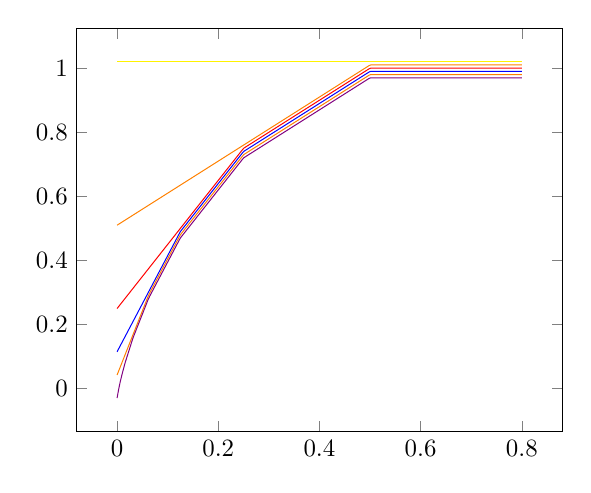
\begin{tikzpicture}[scale=0.9]
\begin{axis}[samples=250]
\addplot[yellow,domain=0:0.8] {1+0.02};

\addplot[orange,domain=0:0.8] {min(x+1/2, 1)+0.01};


\addplot[red,domain=0:0.8] {min(2*x+1/4, x+1/2, 1};
\addplot[blue,domain=0:0.8] {min(3*x+1/8,2*x+1/4, x+1/2, 1)-0.01};
\addplot[orange,domain=0:0.8] {min(4*x+1/16,3*x+1/8,2*x+1/4, x+1/2, 1)-0.02};

\addplot[violet,domain=0:0.8] {min(
10*x+1/1424,
9*x+1/712,
8*x+1/356,
7*x+1/128,
6*x+1/64,
5*x+1/32,
4*x+1/16,3*x+1/8,2*x+1/4, x+1/2, 1)-.03};


\end{axis}

\end{tikzpicture}
\caption{\small Tropical polynomials $\varphi_0,\dots,\varphi_4$ (top to bottom), and the limit tLs $\varphi$ (in violet). The points where the slope changes are  the tropical roots of $\varphi$, i.e.~the points $x=2^{-(i+1)}$, satisfying $ix+2^{-i}=(i+1)x+2^{-(i+1)}$.}
\label{fig:plot1}%\end{figure}%
\end{wrapfigure} %%

A \emph{tropical root} of a tropical polynomials $\varphi$ is a point $x\in \Lawv$ where $\varphi$ is not differentiable (i.e.~where the slope of $\varphi$ changes), or equivalently, where the minimum defining $\varphi$ is attained at least twice (see \autoref{fig:plot1}).
%For instance, the tropical roots of $\varphi_{n+1}$ are of the form $2^{-(i+1)}$, for $0\leq i \leq n$.
Tropical roots yield the usual factorization property of roots: if $x_{0}$ is a root of $f$, this factorizes as
$f(x)=k\min\{x,x_{0}\}+ g(x)$. Yet, unlike in standard algebra, tropical roots can be computed in linear time \cite{Noferini2015}.
%Tropical polynomials and their roots are the main object of study of tropical geometry.
%
%A
% simple calculation shows that this condition corresponds, in the tropical setting, to the usual notion of root. 

A \emph{tropical Laurent series} of one variable is a function $f:\Lawv\to\Lawv$ of shape $f(x)=\inf_{n\in\N}\{nx+\matr f_{n}\}$, with $\matr  f_{n}\in\Lawv$.
In other words, it is a ``limit'' of tropical polynomials of higher and higher degree.
E.g., the tLs $\varphi(x):=\inf_{n\in\N}\set{nx+2^{-n}}$ (see Fig.~\ref{fig:plot1}) %that we will take as our running example, 
is the ``limit'' of the polynomials $\varphi_{n}$.
Since $\inf$s are not in general $\min$s, the behaviour of tLS may be less predictable than that of tropical polynomials~\cite{Porzio2021}. %For instance, tropical roots for tLs (see \cite{Porzio2021}) may also include limit points of their domain.

%
%
%We will take as our running example
%%given respectively by Equation~\ref{eq:polytrop} and Equation~\ref{eq:defTLS}.
%A positive $x\in[0,\infty)$ is said to be a (finite) \emph{tropical root} of a tropical Laurent series $f:\Lawv\to\Lawv$ iff $f$ is not differentiable at $x$ (w.r.t.\ the usual topology on $\BB R_{\geq0}$.This is equivalent to ask that the $\inf$ defining $f$ at $x$ is obtained \emph{at least} twice.{\color{red} \`e vero anche per TLS o solo per poly questo? Inoltre, Robol parla anche di finite end-points of the domain: nel nostro caso sarebbe $x=0$}

%\begin{example}\label{ex:famous_ex}
% The function $f:\Lawv\to\Lawv$ defined by $f(x):=\inf\limits_{n\in\N}\set{nx+\frac{1}{2^n}}$ is a tropical Laurent series.
%\end{example}

%By plotting its graph {\color{red}vogliamo plottarlo?}, we observe several properties that we will lift to the more general case that we will consider in the next lines, and this example will serve as running one.

Tropical Laurent series arise from a general categorical construction:
it is well known that $\LREL$ admits a comonad $!$ which acts, on objects, by taking the finite multisets, and remember that the coKleisli category $\C C_!$ of a category $\C C$ w.r.t.\ a comonad $!$ is the category whose elements are the same of $\C C$, and $\HOM{\C C_!}{X}{Y}:=\HOM{\C C}{!X}{Y}$, with composition $\circ_!$ defined by making use of the co-multiplication of $!$.
%We will explicit this constructions in our tropical setting in the next lines.
Now, although a matrix $t\in\HOM{\LREL_!}{X}{Y}$ yields a linear map $\Lawv^{!X}\to\Lawv^Y$, by exploiting the coKleisli structure we can also ``express it in the base $X$'', i.e.\ see it as a \emph{non-linear} map $t^!:\Lawv^X\to\Lawv^Y$, by setting $t^!(x):=t\circ_! x$. %(we are identifying $\Lawv^X$ with the set $\HOM{\LREL_!}{\emptyset}{X}$ of the \emph{points} of $X$).
Concretely, we have $t^!(x)_b=\inf_{\mu\in !X} \set{\mu x+ t_{\mu,b}}$, where $\mu x:=\sum_{a\in X} \mu(a)x_a$.
%\begin{remark}%[Tropical Laurent series]
These functions corresponds then to tLs with \emph{possibly infinitely} many variables (in fact, as many as the elements of $X$), %In the following we will also refer to them as tLs. 
% We will call them simply \emph{tropical Laurent series (tLs)}.
% %Since in the general case of $\QREL$, $t^!$ is a Laurent series with operations in $Q$, let us call \emph{tropical Laurent series} the functions of shape $t^!$ for some $t\in\HOM{\LREL_!}{X}{Y}$.
%\end{remark}
%
%We find the usual notion of tLs of one variable as follows:
%\begin{remark}
and by identifying $!\set{*}\simeq \N$ and $\Lawv^{\set{*}}\simeq\Lawv$, the tLs generated by the morphisms in $\HOM{\LREL_!}{\set{*}}{\set{*}}$ are exactly the %functions $f:\Lawv\to\Lawv$ of shape $f(x)=\inf_{n\in\N}\set{nx+\matr f(n)}$, for some $\matr f:\N\to\Lawv$, i.e.\ we recover the 
usual tLs's of one variable.
% \end{remark}

In a similar way, tLs
$f:\Lawv^X\to\Lawv^Y$ 
 with \emph{finite} supports $\C F_b=\set{\mu\in!X\mid\matr f_{\mu,b}\neq\infty}$, and which have thus shape $f(x)_b=\min_{\mu\in\C F} \set{\mu x+ t_{\mu,b}}$, are generalisation of usual tropical polynomials to the case of possibly infinitely many variables.

%\end{align}
%where $+$ is the multiset union.

%Remember that in $\Lawv$ the neutral element for addition is $\infty$ and the neutral for multiplication is $0$, so for instance the evaluation map is the matrix $\RM{eval}^{X,Y}\in\Lawv^{!((X\multimap Y) \times X)\times Y}\simeq\Lawv^{(!!X\times !Y\times !X)\times Y}$ given by $\RM{eval}^{X,Y}_{\rho_1\oplus\rho_2\oplus\mu,b}:=0$ if $\rho_1=[\mu]$ and $\rho_2=[b]$, and $\RM{eval}^{X,Y}_{\rho_1\oplus\rho_2\oplus\mu,b}:=\infty$ otherwise.

\begin{remark}
 There is a clear and well-known relation between tropical polynomial/power series and usual polynomials/power series:
fix a (formal) power series $f=\sum_{i\in I\subseteq\N} a_i x^i$ (polynomials being the case for $I$ finite) with coefficitents $a_i$ in a semiring $Q$;
fix a \emph{valuation} $\mathrm{val}:Q\to \Lawv$.
Then one defines the \emph{tropicalisation} $\trop f:\Lawv \to \Lawv$ of $f$ as $\trop f(\alpha):=\inf_{i\in I} \set{\mathrm{val}(a_i)+i\alpha}$.
Often, if $Q=[0,1]$, one takes as valuation $\mathrm{val}(a)=-\log a$.
\end{remark}

\subsection{Probabilities and a worked out motivational example}\label{sec:proba}

General discussion: optimization properties behave in a Lipschitz way.


- differential privacy and Lipschitzness


- log-probabilities and tropical roots 


- counting computation steps (from Manzonetto, but add relational ``Lipschitz'' reasoning)


- measuring duplications of discrete functions (needs finiteness!)







\section{The category $\LREL$}\label{section3}

\subsection{... As tropical linear/non-linear algebra}


For $Q$ a continuous semiring, one lets the category $\QREL$ (\cite{Manzo2013} calls it $Q^\Pi$) have sets as objects and set-indexed matrices with coefficients in $Q$ as morphisms, i.e.~$\QREL(X,Y):=Q^{X\times Y}$.
%The identity morphism of $\QREL$ is the identity matrix $I\in Q^{X\times X}$,
% given by $i_{a,a}=1$ and $i_{a,b\neq a}=0$, and
The composition $st\in Q^{X\times Z}$ of $t\in Q^{X\times Y}$ and $s\in Q^{Y\times Z}$ is given by $(st)_{a,c}:=\sum_{b\in Y} s_{b,c}t_{a,b}$ (such series converges because $Q$ is continuous).
As expected, $Q^X$ is a $Q$-semimodule and we identify $\HOM{\QREL}{X}{Y}$ with the set of linear maps from $Q^X$ to $Q^Y$, which have shape $f(x)_b=:\sum_{a\in X} \matr f_{a,b}x_a$, for some matrix $\matr f\in Q^{X\times Y}$.
% \begin{remark}
 %Following \cite{Manzo2013, Hofmann2014, Ehrhard2005}, we chose to see a matrix $t$ from $X$ to $Y$ as a map $t:X\times Y\to Q$.
% 
% fix $\HOM{\QREL}{X}{Y}:=Q^{X\times Y}$ with composition $st:X\times Z\to Q$ of $s:Y\times Z\to Q$ and $t:X\times Y\to Q$ defined by $(st)_{a,c}:=\sum_{b\in Y} s_{b,c}t_{a,b}$.
Notice that usual linear algebra conventions correspond to work in $\QREL^{\op}$, %a matrix $X\times Y\to Q$ is usually called a ``$Y\times X$-matrix'', meaning $Y$ rows and $X$ columns
e.g.\ the usual matrix-vector product defines a map $Q^Y\to Q^X$.
Following \cite{Manzo2013, Hofmann2014, Ehrhard2005}, we are instead working with transpose matrices.
%\end{remark}
%
%In $\QREL^{op}$ (which corresponds to systematically taking transpose matrices), composition coincides with the product matrix/matrix and $\hat{(\cdot)}$ with the product matrix/vector.
%In order to avoid confusion, we will refer to a $t\in Q^{X\times Y}$ just as a \emph{matrix from $X$ to $Y$}.
%
%
%
%We must fix a convention for matrices: following \cite{Manzo2013, Hofmann2014, Ehrhard2005}, we fix $\HOM{\QREL}{X}{Y}:=Q^{X\times Y}$ with composition $st:X\times Z\to Q$ of $s:Y\times Z\to Q$ and $t:X\times Y\to Q$ defined by $(st)_{a,c}:=\sum_{b\in Y} s_{b,c}t_{a,b}$.
%In linear algebra, a map $X\times Y\to Q$ is usually called a ``$Y\times X$-matrix'', meaning $Y$ rows and $X$ columns.
%In particular, the product of such a matrix for a vector defines a map $Q^Y\to Q^X$.
%Instead, we prefer to see a $t\in\HOM{\QREL}{X}{Y}$ as giving rise to a map $\hat t:Q^X\to Q^Y$ defined by $\hat t(x)_a:=\sum_{b\in Y} t_{a,b}x_a$.
%In $\QREL^{op}$ (which corresponds to systematically taking transpose matrices), composition coincides with the product matrix/matrix and $\hat{(\cdot)}$ with the product matrix/vector.
%In order to avoid confusion, we will refer to a $t\in Q^{X\times Y}$ just as a \emph{matrix from $X$ to $Y$}.
%As it is expected, $Q^X$ is a $Q$-semimodule and the bijection $\hat{(\cdot)}$ identifies $\HOM{\QREL}{X}{Y}$ with the set of linear maps from $Q^X$ to $Q^Y$.

The main actor of this paper is the category $\LREL$. % of sets and matrices with values over $\Lawv$ (which is a continuous semi-ring).
%, where $\Lawv$ is the already introduced Lawvere quantale, seen as the idempotent complete semiring $(\BB R_{\geq0}\cup\set{\infty},\inf,\infty,+,0)$.
%The category $\LREL$ is well-defined because $\Lawv$ is a continuous semiring (w.r.t.\ its quantale order $\preceq$.
%This amounts to check that $\min$ and $+$ commute with the $\inf$ (as operations on $\BB R_{\geq0}\cup\set{\infty}$, which is immediate), and that $(\Lawv,\preceq)$ is a cpo with $\infty$ as bottom element (which is immediate since in $\Lawv$ we have $\vee = \inf$) .
It is worth observing that the composition in $\LREL$ %is the tropicalisation of the one defining it in $\QREL$, i.e.
reads as \ $(st)_{a,c}:=\inf_{b\in Y}\set{s_{b,c}+t_{a,b}}$;
similarly, the linear functions $f:\Lawv^X\to \Lawv^Y$, %induced by matrices
which we call \emph{tropical linear}, are exactly those of shape $f(x)_b=\inf_{a\in X} \set{\matr f_{a,b}+x_a}$, for some $\matr f\in\Lawv^{X\times Y}$.
%\end{remark}

Tropical Laurent series arise from a general categorical construction:
it is well known that $\LREL$ admits a comonad $!$ which acts, on objects, by taking the finite multisets, and remember that the coKleisli category $\C C_!$ of a category $\C C$ w.r.t.\ a comonad $!$ is the category whose elements are the same of $\C C$, and $\HOM{\C C_!}{X}{Y}:=\HOM{\C C}{!X}{Y}$, with composition $\circ_!$ defined by making use of the co-multiplication of $!$.
%We will explicit this constructions in our tropical setting in the next lines.
Now, although a matrix $t\in\HOM{\LREL_!}{X}{Y}$ yields a linear map $\Lawv^{!X}\to\Lawv^Y$, by exploiting the coKleisli structure we can also ``express it in the base $X$'', i.e.\ see it as a \emph{non-linear} map $t^!:\Lawv^X\to\Lawv^Y$, by setting $t^!(x):=t\circ_! x$. %(we are identifying $\Lawv^X$ with the set $\HOM{\LREL_!}{\emptyset}{X}$ of the \emph{points} of $X$).
Concretely, we have $t^!(x)_b=\inf_{\mu\in !X} \set{\mu x+ t_{\mu,b}}$, where $\mu x:=\sum_{a\in X} \mu(a)x_a$.
%\begin{remark}%[Tropical Laurent series]
These functions corresponds then to tLs with \emph{possibly infinitely} many variables (in fact, as many as the elements of $X$), %In the following we will also refer to them as tLs. 
% We will call them simply \emph{tropical Laurent series (tLs)}.
% %Since in the general case of $\QREL$, $t^!$ is a Laurent series with operations in $Q$, let us call \emph{tropical Laurent series} the functions of shape $t^!$ for some $t\in\HOM{\LREL_!}{X}{Y}$.
%\end{remark}
%
%We find the usual notion of tLs of one variable as follows:
%\begin{remark}
and by identifying $!\set{*}\simeq \N$ and $\Lawv^{\set{*}}\simeq\Lawv$, the tLs generated by the morphisms in $\HOM{\LREL_!}{\set{*}}{\set{*}}$ are exactly the %functions $f:\Lawv\to\Lawv$ of shape $f(x)=\inf_{n\in\N}\set{nx+\matr f(n)}$, for some $\matr f:\N\to\Lawv$, i.e.\ we recover the 
usual tLs's of one variable.
% \end{remark}

In a similar way, tLs
$f:\Lawv^X\to\Lawv^Y$ 
 with \emph{finite} supports $\C F_b=\set{\mu\in!X\mid\matr f_{\mu,b}\neq\infty}$, and which have thus shape $f(x)_b=\min_{\mu\in\C F} \set{\mu x+ t_{\mu,b}}$, are generalisation of usual tropical polynomials to the case of possibly infinitely many variables.

%\end{align}
%where $+$ is the multiset union.

%Remember that in $\Lawv$ the neutral element for addition is $\infty$ and the neutral for multiplication is $0$, so for instance the evaluation map is the matrix $\RM{eval}^{X,Y}\in\Lawv^{!((X\multimap Y) \times X)\times Y}\simeq\Lawv^{(!!X\times !Y\times !X)\times Y}$ given by $\RM{eval}^{X,Y}_{\rho_1\oplus\rho_2\oplus\mu,b}:=0$ if $\rho_1=[\mu]$ and $\rho_2=[b]$, and $\RM{eval}^{X,Y}_{\rho_1\oplus\rho_2\oplus\mu,b}:=\infty$ otherwise.

\begin{remark}
 Let $X$, $Y$ be sets and let $\langle \_,\_\rangle:X\times Y \to \mathbb{R}$.
 For $f:X\to \mathbb R$, define $f^*:Y\to \mathbb R$ by $f^*(y):= \sup_{x\in X}\{\langle x,y\rangle - f(x)\}$.
 Then for $X=!A$, $Y=\Lawv^A$, where $A$ is a set, and $\langle \mu, y \rangle:= \mu y$, we have that $f^!(y)=(-f)^*(-y)$ for all $f\in\Lawv^{!A}$.
 This is precisely the same formal construction yielding the well-known convex conjugate $f^*$ of a function $f$, by taking $X$ any vector space, $Y$ its dual space, and $\langle \_,\_\rangle$ the application bilinear form (acting as the scalar product on coordinates).
 This construction is in turn a generalisation of the Legendre transformation.
 Despite the formal constructions being the same, we ignore for the moment if these could be connected to the study of high-order programs in our setting.
\end{remark}


\subsection{... As tropical weighted relational semantics for high-order languages}

The category $\LREL$ satisfies many nice properties which make it able to model all the variants of the $\lambda$-calculi to which we are interested in here. Although the majority of such properties are shared with the general class of models of $\lambda$-calculi called \emph{weighted relational models}, thoroughly studied in \cite{Manzo2013}, we mention them for our particular case in order to highlight how these look like in the tropical setting, but also to make the non-expert in such topics reader able to follow.
The real interest in our particular model will come in the next \autoref{sec:tls}.


\paragraph*{Prohibited duplication/erasure: the \emph{linear} $\STLC$}\label{sec:3A}
The linear simply typed $\lam$-calculus is a restriction of the ordinary $\lam$-calculus in which programs can only use their arguments \emph{exactly once}.
This is the notion of linearity taken into account by linear logic, and indeed this calculus can be embedded in its \emph{intuitionistic multiplicative} fragment \emph{IMLL}.

More precisely, the linear $\lam$-calculus is obtained from the ordinary one by adding the constraint that each $\lam$-abstracted variable appears exactly once in the scope of the $\lam$-abstraction.

In order to frame it in a category $\C C$, one needs a symmetric tensor product $\otimes$ together with internal hom-set objects $X\multimap Y$ s.t.\ the evaluation and curry maps yield a \emph{symmetric monoidal adjunction}: $\C C(Z\otimes X, Y) \simeq \C C (Z, X\multimap Y)$.
This gives the notion of Symmetric Monoidal Closed Category (SMCC).

[Section III.A, \cite{Manzo2013}], immediately gives:

\begin{fact}\label{fact:LREL_SMCC}
 $\LREL$ is a SMCC, thus a model of the linear $\STLC$.
\end{fact}

Its monoidal structure is given by a tensor product $\otimes$ acting on the objects as the Cartesian product of sets, and as the \emph{Kronecker product}
 %{(\color{red} Ref?)} 
 of matrices on morphisms.
Its closed structures is also given by the Cartesian product on sets, with the usual evaluation and curry maps.
Actually, the SMCC $\LREL$ is even a model of IMLL.


\paragraph*{Allowed duplication/erasure: the $\STLC$ and the probabilistic $\lambda$-calculus $\STLC_\oplus$}\label{sec:STLC+STLCO}

%\subsubsection{Unbounded duplications}

\begin{comment}

In order to interpret the full $\STLC$, we need a Cartesian closed category (CCC).
It is well-known \cite{Mellies2009} that it is always possible to construct a CCC by taking the \emph{co-Kleisli} $\C C_!$ of a so-called \emph{Lafont category} $\C C$.
%, a construction we now quickly recall.
%defined via a \emph{Lafont exponential} comonad $!$.
%Let us quickly recall the ideas behind these notions.
A SMCC is Lafont when it has finite products and it is equipped with a comonad $!$ (its \emph{Lafont exponential}) which, at level of objects, sends $X$ to an object $!X$ being the free commutative comonoid on $X$.
Such objects $!X$ represent the \emph{bang} connective of linear logic, granting infinite duplications via the infinite product $X^0\otimes X\otimes X^2\otimes X^3\otimes\cdots$, each factor representing a possible number of duplications.
It is well-known that, under mild conditions satisfied by $\QREL$, one can explicit this idea via the fact that the map $X\mapsto \finMS{X}$ (where $\finMS{X}$ is the set of finite multi-sets on $X$) lifts to a functor $!:\QREL\to\QREL$ which is a Lafont-exponential comonad.
Specializing [Corollary III.6, \cite{Manzo2013}] to our case, we have:

\begin{proposition}
 $\LREL$ is Lafont.
\end{proposition}

\end{comment}

Let us recall that the coKleisli category $\C C_!$ of a category $\C C$ w.r.t.\ a comonad $!$ is the category whose elements are the same of $\C C$, and $\HOM{\C C_!}{X}{Y}:=\HOM{\C C}{!X}{Y}$, with composition $\circ_!$ defined by making use of the co-multiplication of $!$.
%We will explicit this constructions in our tropical setting in the next lines.
As well-known, if a SMCC is \emph{Lafont}, then one obtains a CCC from it by defining the exponential objects as $X\to Y:=!X \multimap Y$.
With no surprise $\LREL$ is Lafont (\cite[Corollary III.6]{Manzo2013}) and specialising \cite[Theorem III.7]{Manzo2013} we have indeed that the coKleisli $\LREL_!$ is CCC, i.e.\ a model of $\STLC$, where as usual $!$ acts on objects by taking the set of finite multisets.
%It is instructive what its CCC-structure looks like in our tropical world.
The cartesian product of $\LREL_!$ (and of $\LREL$) is the disjoint union $+$ of sets, the \emph{evaluation} morphisms are matrices in $\Lawv^{!(!X\times Y)+X)\times Y}$, and the coKleisli composition of $s\in\Lawv^{!Y\times Z}$ and $t\in\Lawv^{!X\times Y}$ is the matrix $s\circ_! t\in\Lawv^{!X\times Z}$ where $(s\circ_! t)_{\mu,c}:=
%\begin{align}
\inf_{n\in\N, b_1\dots,b_n\in Y, \mu = \mu_1+\cdots +\mu_n}
 \left\{s_{[b_1,\dots,b_n],c} + \sum_{i=1}^n t_{\mu_i,b_i}\right\}$.
%\end{align}
%where $+$ is the multiset union.

%Remember that in $\Lawv$ the neutral element for addition is $\infty$ and the neutral for multiplication is $0$, so for instance the evaluation map is the matrix $\RM{eval}^{X,Y}\in\Lawv^{!((X\multimap Y) \times X)\times Y}\simeq\Lawv^{(!!X\times !Y\times !X)\times Y}$ given by $\RM{eval}^{X,Y}_{\rho_1\oplus\rho_2\oplus\mu,b}:=0$ if $\rho_1=[\mu]$ and $\rho_2=[b]$, and $\RM{eval}^{X,Y}_{\rho_1\oplus\rho_2\oplus\mu,b}:=\infty$ otherwise.

%As it is well-known, the Cartesian closed structure %of a category $\C C$  allows to define a sound interpretation $\model{\Gamma\vdash M:A}\in\HOM{\LREL_{!}}{\model \Gamma}{\model A}$ of terms as morphisms.
%In our case, we have:







%Recall the two approaches with more details on lambda-calculus and on existing challenges.


%In this section, we discuss in some more detail the two approaches to quantitative semantics we mentioned in the Introduction, at the same time providing an overview of how we aim at bridging them using tropical mathematics.

\paragraph*{Controlled duplication/erasure via graded types: bounded $\lambda$-calculus $\BSTLC$}\label{sec:BSTLC}

One can see that the comonad $!$ of $\LREL$ can be ``decomposed'' {\color{red}REF} into a family of ``graded exponentials functors'' $!_n:\LREL\to\LREL$ ($n\in\BB N$), defined on objects by taking multisets of cardinality \emph{at most} $n$. %  lift to functors 
The sequence $(!_n)_{n\in\N}$ gives rise to a so-called \emph{$\N$-graded linear exponential comonad} on (the SMC) $\LREL$. %satisfying the adjunction: $\LREL(Z\otimes !_{n}X,Y) \simeq \LREL(Z, !_{n}X\multimap Y)$.

As such, $(\LREL,(!_n)_{n\in\N})$ is a model of graded calculi ensuring bounded duplications via graded typing systems, for instance it is a model  \cite{Katsumata2018} of the language $\BSTLC$, a simplified version of the language $\mathrm{Fuzz}$ \cite{Reed2010}, defined as follows: 
the terms are as for the $\STLC$, the types are $A::= * \ \mid  \ !_{n}A \multimap A$, the contexts of the typing judgements are sets of declarations of the form $x :_{n}A$, with $n\in \mathbb N$, and the typing rules are: %given in Fig.~\ref{fig:rules}
	\[ \scriptsize \arraycolsep=5pt\def\arraystretch{2.8}
	\begin{array}{cccc}
		\prooftree
		\Gamma \vdash M:A
		\justifies
		\Gamma, x:_{0}B \vdash M:A
		\endprooftree 
		&
		\prooftree
		\Gamma, x:_{n}B, y:_{m} B\vdash M:A
		\justifies
		\Gamma, x:_{n+m}B\vdash M\{x/y\}:A
		\endprooftree 
		&
		\prooftree
		\Gamma, x:_{n} A\vdash M: B
		\justifies
		\Gamma\vdash \lambda x.M: !_{n}A\multimap B
		\endprooftree
		&
		\prooftree
		\Gamma \vdash M: !_nA\multimap B
		\quad
		\Delta\vdash N: A
		\justifies
		\Gamma +n\Delta\vdash MN: B
		\endprooftree
	\end{array}
	\]
where $\Gamma+\Delta$ is defined letting $(\Gamma, x:_{m} A)+( \Delta, x:_{n} A) =  (\Gamma+\Delta), x:_{m+n}A$, and $m\Gamma$ is made all $x:_{mn}A$ for $(x:_{n}A) \in \Gamma$.  
The axiom is $x:_{1}A\vdash x: A$.
The main feature of this language is that if $\vdash \lambda x.M:\,!_nA\multimap B$, then $x$ is duplicated at most $n$ times in the reduction of $\vdash (\lambda x.M)N :B$ to the normal form.
%E.g., $\vdash_{\BSTLC} \lambda {\color{red}z}.\left( \lambda x{\color{green}y}. yxx \right)z : \, !_{\color{red}2} *\multimap !_{\color{green}1}(!_{\color{violet}1} * \multimap !_{\color{blue}1} * \multimap *) \multimap *$.
%Observe that one can always type an affine term like e.g.~$\lambda xy.x$ with a linear type $A\multimap B\multimap A$. Instead, a term like $\lambda xy.x(xy)$ containing two occurrences of $x$ cannot be given the linear type $(A\multimap A)\multimap (A\multimap A)$ but a type of the form
%$!_{2}(A\multimap A)\multimap (A\multimap A)$. 

%\begin{remark}\label{rmk:ModelsOfBSTLC}
%Similarly to It is known {\color{red}(([reference??] e dire meglio)} 

Remark that since arrow types are interpreted via $\model{!_{n}A\multimap B}:= !_{n}\model A \times \model B$, 
if $\model *$ is finite, then $\model{A}$ is a finite set for any type $A$ of $\BSTLC$.
%\end{remark}
%Bounded types are interesting because of the following proposition:
%\begin{proposition}
%For all bounded types $A,B$, the morphisms from $\model A$ to $\model B$ (in all parametric relational models) correspond to polynomials.
%\end{proposition}
%\begin{proof}
%It suffices to check that $\model A$ is finite for all bounded types $A$. Indeed this implies that a morphism $t:\model A\to \model B$ is a finite matrix $t: \model A \times \model B \to \Lawv$.Hence, its corresponding map $\widehat t:\Lawv^{\model A} \to \Lawv^{\model B}$ is a polynomial.
%\end{proof}

%For example (here $!_{n}(\Lawv^{X}):= \Lawv^{\C M_{\leq n}(X)}$):
%\begin{itemize}
%\item a map $f\in \LREL( !_{1}\Lawv, \Lawv)$ is of the form $f(x)=\min \{x+a,b\}$;
%\item a map $f\in \LREL(!_{2}\Lawv, \Lawv)$ is a ``quadratic'' polynomial $f(x)=\min\{2x+a, x+b, c\}$.
%\end{itemize}

\begin{comment}

\begin{figure*}

	\scriptsize
	
	\[ \arraycolsep=5pt\def\arraystretch{2.8}
	\begin{array}{cccc}
		\prooftree
		\Gamma \vdash M:A
		\justifies
		\Gamma, x:_{0}B \vdash M:A
		\endprooftree 
		&
		\prooftree
		\Gamma, x:_{n}B, y:_{m} B\vdash M:A
		\justifies
		\Gamma, x:_{n+m}B\vdash M\{x/y\}:A
		\endprooftree 
		&
		\prooftree
		\Gamma, x:_{n} A\vdash M: B
		\justifies
		\Gamma\vdash \lambda x.M: !_{n}A\multimap B
		\endprooftree
		&
		\prooftree
		\Gamma \vdash M: !_nA\multimap B
		\quad
		\Delta\vdash N: A
		\justifies
		\Gamma +n\Delta\vdash MN: B
		\endprooftree
		\\
		\\
		\hline
		\\
		\prooftree
		\Gamma, x: A\vdash M: B
		\justifies
		\Gamma\vdash \lambda x.M: A\to B
		\endprooftree 
		&
		\prooftree
		\Gamma \vdash M: A\to B
		\quad
		\Gamma\vdash \mathbb T: A
		\justifies
		\Gamma \vdash M\mathbb T: B
		\endprooftree 
		&
		\prooftree
		\Gamma \vdash M: A\to B
		\quad
		\Gamma \vdash N: A
		\justifies
		\Gamma \vdash \Diff{M}{N}: A\to B
		\endprooftree
		&
		\prooftree
		\Gamma\vdash M_1: A
		\,\cdots\,
		\Gamma \vdash M_n:A
		\justifies
		\Gamma \vdash M_1+\cdots +M_n : A
		\using (n\geq 2)
		\endprooftree
	\end{array}
	\]
	\caption{Typing rules (axiom rules are given in the text) for $\BSTLC$ (top) and $\STDLC$ (bottom).}\label{fig:rules}
\end{figure*}

\end{comment}

\paragraph*{Controlled duplication/erasure via resources: the differential $\lambda$-calculus $\STDLC$}\label{sec:STDLC}

A Cartesian closed differential $\lambda$-category (CC$\partial\lambda$C)\cite{Manzo2010,Blute2009, Blute2019} is a CCC enriched over commutative monoids %(i.e.\ we can add morphisms and there is a $0$ morphism)
%, it is Cartesian closed%(with the closed structure compatible with the additive structure)
and equipped with a certain \emph{differential operator} $D$, generalising the usual notion of differential, see e.g.\ \cite{BluteEhrhTass10}.
%An example is the CC$\partial\lambda$C of convenient vector spaces with smooth maps, where $D$ is the ``real'' differential $Df:\mathbb{V}\times\mathbb{V}\rightarrow \mathbb{W}$, $Df(x,u):=\dfrac{d}{dt}{\!\Big|_{t=0}} f(x+tu)$, of smooth maps $f:\mathbb{V}\rightarrow \mathbb{W}$.
%More precisely, a cartesian category $\C C$ is a $C\partial C$ when:
%\begin{itemize}
%\item $\C C$ is left-additive, i.e.~its hom-sets have the structure of commutative monoids, and the cartesian structure is well-behaved w.r.t.~this monoid structure;
%\item $\C C$ is equipped with a differential operator $D:
%\C C(X,Y)\to \C C(X\times X,Y)$ satisfying some axioms which capture usual properties of differentials (e.g.~the linearity of $D$ in one of its two variables, the chain rule, etc.).
%\end{itemize}
Now, applying \cite[Theorem 6.1]{lemay2020} one can check that
%\begin{proposition}[{\color{red}LEMAY??}]\label{thm:LREL!CCDC}
 $\LREL_!$ becomes a CC$\partial\lambda$C when equipped with the \emph{tropical differential operator} $D:\HOM{\LREL}{!X}{Y}\to \HOM{\LREL}{!(X\& X)}{Y}$ defined as $(Dt)_{\mu\oplus\rho,b}=t_{\rho+\mu,b}$ if $\#\mu=1$ and as $\infty$ otherwise (using the iso $(\mu,\rho)\in !Z\times !Z'\mapsto\mu\oplus\rho \in !(Z+Z')$).
%\end{proposition}
%\begin{remark}For $t\in\HOM{\LREL}{!X}{Y}$, we have: $D^2 t\in\HOM{\LREL_!}{(X+X)+(X+X)}{Y}$, where $(D^2 t)_{(\rho\oplus\rho')\oplus(\nu\oplus\nu'),b}$ equals $t_{\nu+\nu'+\rho',b}$ if $\rho=\emptyset$ and $\#\rho'=1=\#\nu$; it equals $t_{\rho+\nu',b}$ if $\rho'=\emptyset=\nu$ and $\#\rho=1$; it equals $\infty$ otherwise.\end{remark}
%This ensures that one can define a sound interpretation of $\STDLC$-terms in the standard way (see [Section 4.3, \cite{Manzo2010}]).

As such, $(\LREL_!,D)$ is a model of the differential $\lambda$-calculus $\STDLC$ \cite{ER}, a language ensuring exact control of duplications via a notion of linear substitution.
Its syntax (e.g.\ \cite[Section 3]{Manzo2010}) is given by the \emph{terms} $M$ and the \emph{sums} $\mathbb T$, mutually generated by: $M::= x\mid \lambda x.M \mid M\mathbb T \mid \Diff{M}{M}$ and $\mathbb T::= 0 \mid M \mid M+\mathbb T$,
quotiented by $\alpha$-equivalence, by equations that make $+,0$ form a commutative monoid on the set of sums, %, i.e.\ commutativity and associativity of $+$ and neutrality of $0$ w.r.t.\ $+$;
by linearity of $\lam x.(\_)$, $\Diff{\_}{\_}$ and $(\_)\mathbb T$ (but \emph{not} of $M(\_)$) and by irrelevance of the order of consecutive $\Diff{\_}{\_}$.
%Remark that $M(\_)$ is \emph{not} set to be linear: $\lambda x.0=0\mathbb T=\Diff{0}{N}=\Diff{M}{0}=0$ but $M0\neq0$ in general.
%This is crucial for the definition of the Taylor expansion.
We follow the tradition of quotienting also for the idempotency of $+$.
%Sums are, then, just \emph{finite} sets of terms.
The types are $A::= *\mid A\to A$, the typing rules: %in Figure~\ref{fig:rules}
	\[ \scriptsize \arraycolsep=5pt\def\arraystretch{2.8}
	\begin{array}{cccc}
		\prooftree
		\Gamma, x: A\vdash M: B
		\justifies
		\Gamma\vdash \lambda x.M: A\to B
		\endprooftree 
		&
		\prooftree
		\Gamma \vdash M: A\to B
		\quad
		\Gamma\vdash \mathbb T: A
		\justifies
		\Gamma \vdash M\mathbb T: B
		\endprooftree 
		&
		\prooftree
		\Gamma \vdash M: A\to B
		\quad
		\Gamma \vdash N: A
		\justifies
		\Gamma \vdash \Diff{M}{N}: A\to B
		\endprooftree
		&
		\prooftree
		\Gamma\vdash M_1: A
		\,\cdots\,
		\Gamma \vdash M_n:A
		\justifies
		\Gamma \vdash M_1+\cdots +M_n : A
		\using (n\geq 2)
		\endprooftree
	\end{array}
	\]
where a context $\Gamma$ is a list of typed variable declarations.
The axioms are $\Gamma, x:A \vdash x: A$ and $\Gamma\vdash 0:A$.
The main feature of this language is that $\Der^n[\lambda x.M,N^n]0$ has a non-zero normal form iff $x$ is duplicated exactly $n$ times during the reduction to normal form.
%In $\BSTLC$ the typing system handles duplications; in $\STDLC$ the syntax with its operational semantics (that we do not give) does it.
\begin{comment}
Writing $\Der^2[\_,(\_)^2]$ as a shortcut for $\Der[\Der[\_,\_],\_]$ and $\Der^1[\_,(\_)^1]$ for $\Diff{\_}{\_}$, the analogue of the previous $\BSTLC$-term is $\vdash_{\STDLC} \lambda {\color{red}z}. \Der^{\color{red}2}[
	\lambda x{\color{green}y}.
		\Der^{\color{violet}1} [
				\Der^{\color{blue}1} [y, x^{\color{blue}1}]
        0, x^{\color{violet}1}
	]0
, z^{\color{red}2}]0
: {\color{red}*}\to ({\color{green}* \to * \to *}) \to *$.
%Here we wrote $\Der^2[\_]\cdot (\_)^2$ as a shortcut for $\Der[\Der[\_]\cdot (\_)]\cdot (\_)$ and $\Der^1[\_]\cdot (\_)^1$ for $\Der[\_]\cdot (\_)$.
In particular, if the \emph{multiplicities} of the arguments (the colored exponents) do not exactly match the number of duplications, e.g.\ in $\vdash_{\STDLC} \lambda z. \Der^{\color{red}3}[
	\lambda xy.
		\Diff{
				\Diff{y}{x}
		0}{x}
	0
, z^{\color{red}3}]0
: *\to (* \to * \to *) \to *$, then the term reduces to the empty sum $0$ (representing an \emph{error}).
\end{comment}
%Correspondingly, the syntax of the simply typed \emph{differential} $\lambda$-calculus ($\STDLC$) is defined by enriching $\STLC$ with a monoid structure $0,+$ over terms, as well as with $\Der$ and a notion of \emph{linear substitution} (see \cite{difflambda} or the Appendix for details).

%Until now we simply specialised well-known results in our tropical case, with the intent of showing how things read in this particular case.
%Now we go further, by showing that $\LREL_!$ actually admits a \emph{differential structure}, turning it into a model of the $\STDLC$, i.e.~a $CC\partial C$.
%This viewpoint
%, is where the \emph{metric} and the \emph{differential} viewpoints converge, as explained in the Introduction and Section II, and it % will be further generalised in Section \ref{section6}.

%A model of the $\STDLC$ is usually understood as so-called \emph{Cartesian closed differential categories} (CC$\partial$C), see \cite{Manzo2012} for details.
%In order to treat the $+$ and the constructor $D[\_]\cdot (\_)$ of $\STDLC$, the main features of a CC$\partial$C $\C C$ are that:
%
%1) $\C C$ is a left-additive-CCC, i.e.\ its Homsets are commutative monoids and its Cartesian closed structure is well behaved w.r.t.\ this monoid structure;
%
%2) $\C C$ is equipped with a differential operator map $D:\HOM{\C C}{X}{Y}\to \HOM{\C C}{X\times X}{Y}$ (here $\times$ is the Cartesian product of $\C C$) satisfying $8$ axioms, called D1, ..., D7, D-curry.

%Let us show the differential structure of $\LREL_!$ (remember that the Cartesian product of $\LREL_!$ is the disjoint union $+$).

%\begin{definition} The \emph{tropical differential operator} is the map $D:\HOM{\LREL}{!X}{Y}\to \HOM{\LREL}{!(X+X)}{Y}$ defined as $(Dt)_{\mu\oplus\rho,b}=t_{\rho+\mu,b}$ if $\#\mu=1$ and as $\infty$ otherwise (where a multiset $\nu \in !(X+X)$ is identified with a disjoint sum of $\mu,\rho\in !X$).\end{definition}

%The models of $\STDLC$ are the cartesian \emph{closed} differential categories ($CC\partial C$), which are defined as $C\partial C$ which are also cartesian closed, and in which the monoid structure and the differential operator are both well-behaved with respect to the closed structure \cite{Manzo2012}. 


 



\section{Tropical Laurent Series}\label{sec:tls}
In this section we study the tropical Laurent series $\Lawv^X\to \Lawv ^Y$ from the viewpoint of analysis.

Let us start by recalling Example~\ref{ex:famous_ex}.
By plotting its graph {\color{red}vogliamo plottarlo?}, we see first of all that the function is non-decreasing and concave.
It is easy to see that this is actually always the case:

\begin{proposition}
 Any tropical Laurent series $f:\Lawv^X\to\Lawv^Y$ is non-decreasing and concave, w.r.t.\ the pointwise order.
\end{proposition}

The $f$ of Example~\ref{ex:famous_ex} is continuous on $\BB R_{\geq0}=\Lawv-\set{\infty}$ (w.r.t.\ the usual norm of real numbers).
By considering the usual norm $\norm{x}_\infty:=\sup\limits_{a\in X} \absv{x_a}$ on $\Lawv^X$, we could generalise this property by dropping the case of $x$ having some $0$ coordinate:

\begin{theorem}\label{thm:cont}
 Any tropical Laurent series $f:\Lawv^X\to\Lawv$ is continuous on $\BB R_{>0}$, w.r.t.\ to the norm $\norm{\cdot}_\infty$.
\end{theorem}
\begin{proof}
 The result follows after proving that if a real-valued function on a locally convex topological $\BB R$-vector space is, locally around $x$, concave and bounded by a finite constant, then it is continuous at $x$.
\end{proof}

Not only the $f$ of Example~\ref{ex:famous_ex} is continuous, but it is also locally Lipschitz on $\BB R_{>0}$.
Actually, we can prove the following:

\begin{theorem}
 Let $f:\Lawv\to\Lawv$ a tropical Laurent series with matrix $\widehat f:\N\to\Lawv$.
 For all $0<\epsilon<\infty$, there is a \emph{finite} $\C F_\epsilon \subseteq \N$ s.t.:
 \begin{enumerate}
  \item If $\C F_\epsilon=\emptyset$ then $f=\infty$ on all $\Lawv$;
  \item If $f(x_0)=\infty$ for some $x_0<\infty$, then $\C F_\epsilon=\emptyset$;
  \item On all $[\epsilon,\infty]$, $f$ coincides with the tropical \emph{polynomial} $P_\epsilon(x):=\min\limits_{n\in \C F_\epsilon}\set{nx+\widehat f(n)}$.
 \end{enumerate}
 In particular, $f$ is locally Lipschitz on all $\BB R_{>0}$.
\end{theorem}
\begin{proof}
 We can let $\C F_\epsilon:=\set{n\in\N \mid
 \widehat f(n)<\infty \textit{ and } \widehat f(m)> \widehat f(m)+\epsilon \textit{ for all } m<n}$.
\end{proof}

Remark that, in coherence with the previous result, in Example~\ref{ex:famous_ex} $f(x)$ is indeed a $\min$ for all $x>0$.
At $x=0$ we have $f(x=0)=\inf\limits_{n\in\N} \frac{1}{2^n}=0$ which is \emph{not} a min.
Also, while the derivative of $f$ is bounded on all $\BB R_{>0}$, at $x=0$ it tends to $\infty$.
This phenomenon is reminiscent of [Example 7, PCoh]
%Differentials and Distances in Probabilistic Coherence Spaces. FSCD 2019
, which actually motivated our first investigations.

We could generalise the locally Lipschitz property as follows:
\begin{theorem}
 Let $f:\Lawv^X\to\Lawv$.
 If $f$ is non-decreasing, concave and continuous, then it is locally Lipschitz.
\end{theorem}
\begin{proof}
 Refinement of the arguments used for Theorem~\ref{thm:cont}.
 {\color{red}Che ci scriviamo?}
\end{proof}

Highlight compositional reasoning based on Lipschitz.\\

- the metric on the tensor is the usual tensor metric, the metric on the function space is the usual function metric, the metric on multisets is the multiset metric

{\color{red}
- extend this result to functions $\Lawv^{X}\to \Lawv^{Y}$ with $X,Y$ finite (as this will be useful in section V) Quale ?} 



- discussion of the tropical Taylor expansion: 


- characterization of the functional metric using derivatives\\

Let us end this section by mentioning another point of view on tropical Laurent series.
$\Lawv^X$ with the usual $+$ and the usual $\cdot$ is a $\BB R_{\geq0}$-semimodule.
Together with the norm $\norm{\cdot}_\infty$, it can be proved that it is a Scott-complete normed cone.
The normed cone structure induces an order on it, called its \emph{cone order}, by setting:
$x\leq y$ iff $y=x+z$ for some (unique) $z\in\Lawv^X$.
This order makes it a Scott-continuous dcpo.
Furthermore we have:

\begin{proposition}
  Tropical Laurent series $\Lawv^X\to\Lawv^Y$ are Scott-continuous on $\BB R_{>0}$, w.r.t.\ the cone orders on the domain and codomain.
\end{proposition}



%\section{Future lines of research}\label{sec:future}

%\subsection{Quantitaive analysis}\label{sec:app}
%%

\subsection{Resource Analysis for Differential Privacy}

The typical situation in differential privacy is where one considers a probabilistic query $f: \mathsf{db}\to [0,1]^{X}$ over some database, and one requires that $f$ should not be \emph{too sensitive} to small changes in the output, in other to prevent potential leaks of private information about individual items in $\mathsf{db}$ (for instance, an element $x\in\mathsf{db}$ could be the list of students of some university and $f(x)$ could indicate the percentage of female students$\mathsf{db}$).

More formally, differential privacy is defined as follows:
\begin{definition}
Let $f: \mathsf{db}\to [0,1]^{X}$ and $\epsilon \in \BB R_{\geq 0}$. $f$ is said \emph{$\epsilon$-differentially private} if for all $x,x'\in \mathsf{db}$
differing by $L$ items, for all $s\in X$, 
$
f(x)(s) \ = \ e^{\epsilon L} f(x')(s)
$.
\end{definition}

A well-studied approach to ensure differential privacy for higher-order programs is to use bounded type systems like $\mathsf{Fuzz}$ \cite{Reed2010}. Indeed, such systems come with an \emph{a priori} warrant that well-typed programs are Lipschitz.

Tropical semantics suggests that resource analysis could also be used to provide bounds for differential privacy. 
Suppose our probabilistic query $f$ can be expressed as a power series (this is what happens e.g.~in \emph{probabilistic coherent spaces} \cite{Ehrhard2011}). Then, if we discover, either by studying differential properties of $f$, or by using methods from convex analysis as suggested in the previous section (e.g.~Theorem \ref{theorem:fepsilon}), 
 that the tropicalization $\trop f$ satisfies a Lipschitz condition, we may use this fact to deduce that $f$ is differentially private, as shown by the result below.

%
%We have seen how a higher-order probabilistic program, which is expressed as a polynomial, can be tropicalized. This operation can be extended to programs expressed as power series by taking the limit. 
%

Let us equip the space $[0,1]^{X}$ with the metric $d(x,y)=\sup_{a\in X}|\log x_{a}-\log y_{a}|$. Then we have the following:
\begin{proposition}
Let $f: [0,1]^{X}\to [0,1]^{Y}$ be a function expressed by a power series. If $\trop f$ is $\epsilon$-Lipschitz over some open set $U$, then $f$ is $\epsilon$-differentially private over $\psi_{t}(U)$, for small enough $t$.
\end{proposition}
\begin{proof}[Proof sketch]
%We consider the case $X=Y=\B 1$ for simplicity. 
%Express $f$ as a power series $f(x)=\sum_{n}\psi_{e}(\widehat f_{n})x^{n}$, so that $\trop f(\alpha)= \inf_{n}\left \{
%n\alpha + \widehat f_{n}
%\right\}$.
%Let us define a family of intermediate functions $\trop_{t}f(\alpha)=\phi_{t}(\stackrel{t}{\sum_{n}}\widehat{f}_{n}\times_{t}n\alpha)$. These, by construction, satisfy
%\begin{align}\label{eq:phit}
%f(\phi_{t}(\alpha)) = \phi_{t}(\trop_{t}f(\alpha))
%\end{align}
%and, using the fact that $\alpha\sumt{t}\beta\to\min\{\alpha,\beta\}$ and $\alpha\prodt{t}\beta\to \alpha+\beta$, we can deduce that $\trop f(\alpha)=\lim_{t\to 0}\trop_{t}f(\alpha)$ (for this, we use the fact that for all $m\in \BB N$,
%$\min_{i\leq m}\alpha_{i}\leq \stackrel{t}{\sum}_{i\leq m}\alpha_{i}\leq 
%(\min_{i\leq m}\alpha_{i})+t\log m$).
We consider $X=Y=\{\star\}$ for simplicity.
With the notations from \S \ref{section3}.A, using the fact that $\lim_{t\to 0}\trop_{t}f= \trop f$, as well as the commutation $f(\phi_{t}(\alpha)) = \phi_{t}(\trop_{t}f(\alpha))$ (which follows from the definition of $\trop_{t}$), one can see that the Lipschitz condition  
$|\trop f(\phi_{t}(x))-\trop f(\phi_{t}(y))|\leq \epsilon |\phi_{t}(x)-\phi_{t}(y)|$ translates into the condition 
$f(x) \leq e^{\epsilon |\log x-\log y|} f(y)$ (supposing $y\geq x$ and $f(y)\neq 0$).
\end{proof}

%General discussion: optimization properties behave in a Lipschitz way.
%
%
%- differential privacy and Lipschitzness
%
%
%- log-probabilities and tropical roots 
%
%
%- counting computation steps (from Manzonetto, but add relational ``Lipschitz'' reasoning)
%
%
%- measuring duplications of discrete functions (needs finiteness!)





%\subsection{Generalized Metric Spaces and Modules over the Lawvere Quantale}\label{section6}
%%At the basis of our approach is the observation that the \emph{tropical semiring} $([0,\infty], \min, +)$, which is at the heart of tropical mathematics, coincides with the \emph{Lawvere quantale} $\Lawv=([0,\infty], \geq, +)$ \cite{Hofmann2014, Stubbe2014}, the structure at the heart of the categorical study of metric spaces initiated by Lawvere himself \cite{Lawvere1973}.
%Let us recall that a quantale is a complete lattice endowed with a continuous monoid action. In the case of $\Lawv$ the lattice is defined by the reverse order $\geq$ on $\BB R$, and the monoid action is provided by addition. Notice that the lattice join operation of $\Lawv$ coincides with the idempotent semiring operation $\min$. 
%A consequence of these observations is that, as we discussed below, the tropical approach to linear algebra coincides with the study of ``$\Lawv$-valued matrices'', i.e.~of maps of the form $s: X\times Y\to \Lawv$ .
%In particular, a (possibly $\infty$) metric on a set $X$ is nothing but a ``$\Lawv$-valued square matrix'' $d:X\times X\to \Lawv$ satisfying axioms like e.g.~the triangular law (indeed, such distance matrices correspond to $\Lawv$-\emph{enriched categories}, a viewpoint we explicitly take in Section \ref{section6}). 
%
- correspondence between $\Lawv$-modules and $\Lawv$-categories.


- exponential structure of $\LCAT$.


- $\LCAT_{!}$ is a cartesian closed differential category

%


\section{Related Work}\label{section7} 
The connections between the differential $\lambda$-calculus (and differential linear logic), the relational semantics, and the theory of non-idempotent intersection types is very well-studied (see \cite{}, and more recently, \cite{} for a more abstract perspective, and \cite{} for a 2-categorical, or proof-relevant, extension).
As we said, the relational semantics over the tropical semi-ring was quickly explored in \cite{}, to provide a ``best case'' resource analysis of a $\B{PCF}$-like language with non-deterministic choice. 
\emph{Probabilistic coherent spaces} \cite{}, a variant of  the relational semantics, provide an interpretation of higher-order probabilistic programs
as analytic functions. In \cite{} it was observed that such functions satisfy a local Lipschitz condition somehow reminiscent of our examples in Section \ref{section4}.


The study of linear or bounded type systems for sensitivity analysis was initiated in \cite{} and later developed \cite{}.
As recalled in the paper, the use bounded exponentials ensures that well-typed programs satisfy a Lipschitz condition.
Related approaches, although not based on metrics, are provided by \emph{differential logical relations} \cite{} and \emph{change action} models \cite{}.


More generally, the literature on program metrics in denotational semantics is vast. Since [6] metric spaces, also in Lawvere's generalized sense \cite{}, have been exploited as an alternative framework to standard, domain-theoretic, denotational semantics. 
While standard categories of metric spaces are not models of the full simply typed $\lambda$-calculus, several constructions of cartesian closed categories of metric spaces can be found in the literature. For instance, 
\emph{ultra}-metric spaces \cite{} form a CCC, and have been shown to model $\B{PCF}$ \cite{}.
Also \emph{partial} metrics, introduced in \cite{}, have been shown to provide models of $\STLC$, under suitable generalizations \cite{}.
More generally, \cite{} provides a general characterization of exponentiable objects in categories of (generalized) metric spaces, and \cite{} provides other ways to construct CCCs of
(generalized) metrics, including one based on locally Lipschitz maps, 
using ideas from {differential logical relations}.

Motivated by connections with computer science and fuzzy set-theory, 
the abstract study of generalized metric spaces in the framework of \emph{quantale}- or even \emph{quantaloid}-enriched categories has led to a vast literature in recent years \cite{}, 
and its connections with tropical mathematics are discussed in \cite{}. Moreover, applications of quantale-modules to both logic and computer science have also been studied \cite{}.

Connections between program metrics and the differential $\lambda$-calculus have been already suggested in \cite{}; moreover, \emph{cartesian difference categories} \cite{} have been proposed as a way to relate derivatives in differential categories with those found in change action models.



Finally, applications of tropical mathematics in computer science abound, notably in optimization methods for machine learning \cite{} (typically, for neural networks with peicewise linear activation), linear regression \cite{}, convex analysis \cite{}, as well as finite automata \cite{}.
While our discussion in Section \ref{section5} is inspired by a well-known application of tropical polynomials \cite{},  
the vast literature in this domain lets us think that other ways to 
apply tropical semantics to the analysis of higher-order programs might be studied.

%
%Other connections tropical/metric -> Fuji, ??
%Applications of tropical to computer science.
%Log-probabilities.
%Quantale-modules -> Abramski?
%
%
 












\section{Conclusion and future work}\label{section8} 


In our opinion, the main goals of this paper are two. Firstly,  to
demonstrate the existence of a conceptual bridge between two different well-studied quantitative approaches to higher-order programs, and to highlight the possibility of transferring results and techniques from one approach to the other. 
Secondly, to suggest that tropical mathematics, a
field which has been largely and successfully applied in computer science, could be used to study quantitative properties of higher-order programs.

While the first goal has been developed in detail, and at different levels of abstraction, for the second goal we only sketched a few interesting directions (best-case analysis, log-probabilities, differential privacy). We believe that exploring in more depth these ideas could be a fruitful direction; moreover, 
since both generalized metrics and quantale-modules have been largely applied in computer science, 
a natural question is whether the generalized approach of Section \ref{section6} could  lead to new applications of metric and tropical methods to the $\lambda$-calculus.

Finally, as suggested in Section \ref{section5}, an interesting direction to look at is the semantics of finiteness spaces \cite{Ehrhard2005}, which allows to model typable terms by means of \emph{finitary} Taylor expansions. Indeed, knowing that the application of a program $M$ to $N$ expands as a finite sum of linear applications (hence by a Lipschitz function in our setting), may allow one to predict how sensitive $M$ will be ``around $N$''.
%
%We have shown that:
%
%- intuitively, the interplay between tropical mathematics and $\lam$-calculus \emph{could} relate the metric and differential approaches on approximations of $\lam$-calc (introduction+section 2)
%
%- this relation \emph{can} take place, because the natural category $\LREL$ and its generalised versions are metric models of the differential $\lam$-calculus (section 3 and 6)
%
%- this relation \emph{seems} to provide applications in different fields (section 5).
%
%Therefore, we mainly set the basis for future interplays between all these areas, hopefully motivating the interest in such an interplay.
%For instance, the general questions are:
%
%- Can we improve the results of section 4 ?
%
%- Can we develop and make the applications of section 5 useful ?
%
%- What does the general setting of section 6 give in terms of theoretical and applied results ?
%
%- Do tools from tropical \emph{geometry} provide something for $\lam$-calculus ? (for instance, the role of tropical roots, tropical varieties,...)
%
%- Finally, there is a last point which we think of interest and we did not mention through the paper: the inclusion of finiteness spaces in the picture.
%Say what could they do and why.

%%
%% Bibliography
%%

%% Please use bibtex, 

%\bibliography{tropical}

%\appendix

%\section{\autoref{section3}}\label{app-sec:section3}


\end{document}
